\documentclass[11pt]{article}

\usepackage[margin=1in]{geometry}
\usepackage{graphicx}
\usepackage{booktabs}
\usepackage{amsmath}
\usepackage{amssymb}
\usepackage{hyperref}

\graphicspath{{../data/results/}}

\title{Entropic Stress-Testing of Tool-Using LLM Agents Under Non-Stationary Task Constraints}
\author{[Your Name] \\ [University / Lab] \and [Supervisor/Co-authors] \\ [University / Lab]}
\date{Draft (needs final benchmark runs)}

\begin{document}
\maketitle

\noindent\textbf{Target:} arXiv + [venue TBD]

\begin{abstract}
Current evaluation frameworks for tool-using Large Language Model (LLM) agents largely measure success on fixed objectives (static solvability). In real deployments, objectives can shift mid-execution (non-stationary constraints), and agents can silently fail by persisting with obsolete plans, repeating actions, or ``hallucinating progress''. We introduce an \textbf{Entropic Stress-Test} evaluation harness that injects controlled requirement changes (``shocks'') into deterministic sandboxes and measures agent stability and adaptation. We propose \textbf{Semantic Collapse Ratio (SCR)}, computed via branching probes that sample multiple possible next steps and quantify their semantic divergence, and \textbf{Information Gain Efficiency (IGE)}, a token-cost-normalized uncertainty reduction measure when token logprobs are available. A key practical finding is that logprob-based confidence is frequently unavailable or inconsistent across providers/models; treating missing logprobs as ``0.0 entropy'' is invalid. We show how SCR plus outcome-based validators provide a robust evaluation signal even when token-level confidence is missing, enabling reproducible comparisons across heterogeneous model providers.
\end{abstract}

\section{Introduction}
The rapid adoption of LLM-based agents for autonomous software engineering has highlighted a critical reliability gap. While agents perform well on static benchmarks, their performance degrades significantly in long-horizon tasks with changing requirements. This degradation is often characterized not by immediate failure, but by a gradual ``Context Rot,'' where the agent's internal state drifts from the ground truth, leading to repetitive loops and hallucinated progress.

Standard observability metrics, such as token-level entropy or perplexity proxies, are unreliable in practice: many APIs do not expose token logprobs, and models optimized for helpfulness can produce confident language even when plans are brittle. This creates an observability gap for agent operators: failures may be silent until an external validator fails (or a human notices).

This paper contributes:
\begin{enumerate}
  \item \textbf{A reproducible non-stationary evaluation harness} (orchestrator + deterministic sandboxes + validators) for tool-using agents under controlled requirement shocks.
  \item \textbf{A provider-agnostic stability probe (SCR)}: an active measure of plan instability under shocks via semantic divergence across branched next-step generations.
  \item \textbf{A practical observability result:} entropy proxies derived from token logprobs are often unavailable across providers/models; we therefore report \textbf{entropy coverage} and treat missing entropy as \texttt{null}, not \texttt{0.0}.
  \item \textbf{A secondary behavioral result:} even when entropy is available, it can remain flat/low around shocks while agent behavior destabilizes, whereas SCR spikes near perturbations.
\end{enumerate}

\section{Methodology}

\subsection{System Architecture and Agent Loop}
The Entropic Stress-Test framework has four decoupled components:
\begin{itemize}
  \item \textbf{Orchestrator:} runs the step loop, injects perturbations, and coordinates probes (\texttt{src/orchestrator/core/orchestrator.py}).
  \item \textbf{Sandbox:} deterministic filesystem and command execution (Docker optional with local fallback).
  \item \textbf{Agent:} produces either a tool action or a natural-language reply at each step (\texttt{src/agent/real\_agent.py}).
  \item \textbf{Monitor + Validators:} per-step logging and deterministic success checks (\texttt{src/monitor/terminal\_bench\_monitor.py}, \texttt{src/scenarios/validation\_ops.py}).
\end{itemize}

Each step emits a structured JSONL record with scenario ID, step index, event type, tool call (if any), validator status, token usage, and metrics. Logs are written under \texttt{logs/terminal\_bench/}.

\subsection{Scenario Design and Non-Stationarity}
Each scenario specifies: (1) an initial prompt, (2) a schedule of perturbations (step index plus new instruction), and (3) a validator that checks artifacts in the sandbox. Perturbations are injected as explicit user messages and can optionally mutate sandbox state. This yields deterministic tasks with controlled requirement changes.

The benchmark suite used for paper tables is defined in \texttt{benchmarks/suite\_v2.json} and executed with \texttt{experiments/run\_benchmark.py}.

\subsection{Action Protocol and Token Accounting}
At each step, the agent returns either:
\begin{itemize}
  \item \texttt{tool\_use}: a tool name plus JSON arguments executed in the sandbox, or
  \item \texttt{llm\_reply}: a natural-language response (used on completion or failure).
\end{itemize}

Token usage is recorded when the provider exposes it (\texttt{prompt\_tokens}, \texttt{completion\_tokens}, \texttt{total\_tokens}). Probe calls are tracked separately as \texttt{probe\_total\_tokens} to report totals with and without probes.

\subsection{Branching Probe Protocol}
To measure hidden uncertainty, we run branching probes at perturbation steps and optionally at periodic intervals.
\begin{itemize}
  \item Shock probes: always run at perturbation steps.
  \item Periodic probes: configurable interval (default 5) when no perturbation is triggered.
  \item Branch count: $N$ branches (default 3).
\end{itemize}

Each probe forks the current dialogue state (plus the perturbation message if present) and generates $N$ independent ``next step'' thoughts using a higher temperature (0.9) to encourage divergence. The probe does not execute tools; it only samples candidate next actions for analysis.

\subsection{Metrics}
We report stability and observability metrics that do not depend on a specific provider:

\textbf{Semantic Collapse Ratio (SCR).} We compute SCR as the mean pairwise cosine distance between embedding vectors of the $N$ probe branches:
\[
SCR = \frac{1}{N(N-1)} \sum_{i \ne j} d_{\cos}(v_i, v_j)
\]
where $d_{\cos}$ is cosine distance and $v_i$ are sentence embeddings from a SentenceTransformer model (default \texttt{all-MiniLM-L6-v2}). If embeddings are unavailable, SCR is recorded as null and excluded from summaries.

\textbf{Entropy coverage.} Token logprobs are optional across providers, so we compute entropy only when logprobs are present. We report entropy coverage: the fraction of non-probe steps with entropy values available.

\textbf{Entropy definition (chosen-token proxy).} When logprobs are available, we define entropy as the average negative log probability of the chosen tokens:
\[
H = -\frac{1}{N} \sum_{i=1}^{N} \log p(t_i)
\]
This is a chosen-token surprisal proxy (not full distributional entropy), because most providers do not expose the full token distribution. We therefore always report coverage and treat missing values as null.

\textbf{Information Gain Efficiency (IGE).} When logprobs exist, we compute:
\[
IGE = \frac{H_{pre} - H_{post}}{TokenCost}
\]
where $H$ is the average negative log probability of chosen tokens around a tool action. IGE is undefined when logprobs are absent.

\subsection{Evaluation Protocol}
Each (model, scenario) pair is run for a fixed maximum step budget (default 60 unless overridden by the suite). We repeat each run multiple times (default 3) to estimate variance. Success is determined solely by deterministic validators.

Aggregate metrics are computed with \texttt{analysis/analyze\_benchmark.py} and include success rate, median steps, median token usage, mean entropy coverage, and median peak SCR at perturbation steps.

\section{Experiments}

\subsection{Setup: The ``Drug Filter Shock'' Scenario}
We designed a scenario simulating a real-world data engineering task:
\begin{enumerate}
  \item \textbf{Initial Goal:} Filter \texttt{drugs.csv} by \texttt{weight < 150} and write \texttt{filtered\_by\_weight.csv}.
  \item \textbf{Phase 1 (Steps 1--3):} Agent writes code and generates the CSV.
  \item \textbf{Shock 1 (Step 4):} A ``Manager'' injects a constraint change: the weight filter must now use an external \texttt{get\_molecular\_mass(drug\_name)} API.
  \item \textbf{Shock 2 (Step 7):} The primary filter reverts back to the \texttt{weight} column, but the molecular mass API connection must remain present in code for future use.
\end{enumerate}

\subsection{The ``Rescue'' Protocol}
We include an optional intervention protocol. After persistent ``panic'' (entropy-based when available, loop-based otherwise), the controller can: (a) inject a corrective system message, or (b) in a two-model setup, hand off control to a stronger ``rescue'' model. This protocol is evaluated separately from baseline runs to avoid conflating detection and recovery.

\subsection{Evaluation Outputs (Paper Tables)}
We report:
\begin{itemize}
  \item \textbf{Success rate} (validator pass rate) per (model, scenario)
  \item \textbf{Median steps} to completion / termination
  \item \textbf{Token usage} (including optional probe tokens)
  \item \textbf{Entropy coverage} (fraction of steps with entropy present)
  \item \textbf{Peak SCR at shocks} (median peak SCR over perturbation events)
\end{itemize}

These aggregates are produced by:
\begin{itemize}
  \item \texttt{experiments/run\_benchmark.py} $\rightarrow$ raw results CSV
  \item \texttt{analysis/analyze\_benchmark.py} $\rightarrow$ paper-ready summary CSV
\end{itemize}

Reproducibility runsheet: \texttt{paper/PAPER\_RUNSHEET.md}.

\section{Results}

\subsection{Primary Result: Entropy Coverage Makes ``Entropy-Only'' Observability Non-Viable}
Across providers/models, token logprobs may be missing or inconsistent. As a result, entropy proxies cannot be relied upon as the sole observability signal in multi-provider sweeps. We treat entropy as an optional signal and report \textbf{entropy coverage}: the fraction of non-probe steps with entropy present.

\textbf{Key implication:} any evaluation that compares ``entropy'' across models without reporting coverage is at risk of silently mixing real values with missingness artifacts (e.g., treating missingness as \texttt{0.0}). [CITE]

\subsection{Secondary Result: Entropy Can Decouple from Stability Even When Available}
When token logprobs are available, chosen-token surprisal proxies may remain flat/low around perturbations even as agent behavior becomes unstable (e.g., repeating obsolete plans, oscillating between incompatible actions). In contrast, SCR is designed to measure plan instability directly by quantifying divergence across sampled next steps.

We therefore use SCR as the primary instability indicator around shocks, and entropy (when present) as a complementary, model-specific signal rather than a universal baseline. [CITE]

\subsection{Metric Comparison (Qualitative + Aggregate)}
We analyze metric behavior around perturbation steps. SCR spikes at shocks in scenarios where the agent must revise plans to satisfy new requirements. We report peak SCR at perturbations (median over repeats) as a compact instability summary statistic.

\textbf{TODO (after final runs):} include correlation plots between (SCR at shock, success rate) and (entropy proxy, success rate), and report confidence intervals across repeats.

\begin{figure}[ht]
  \centering
  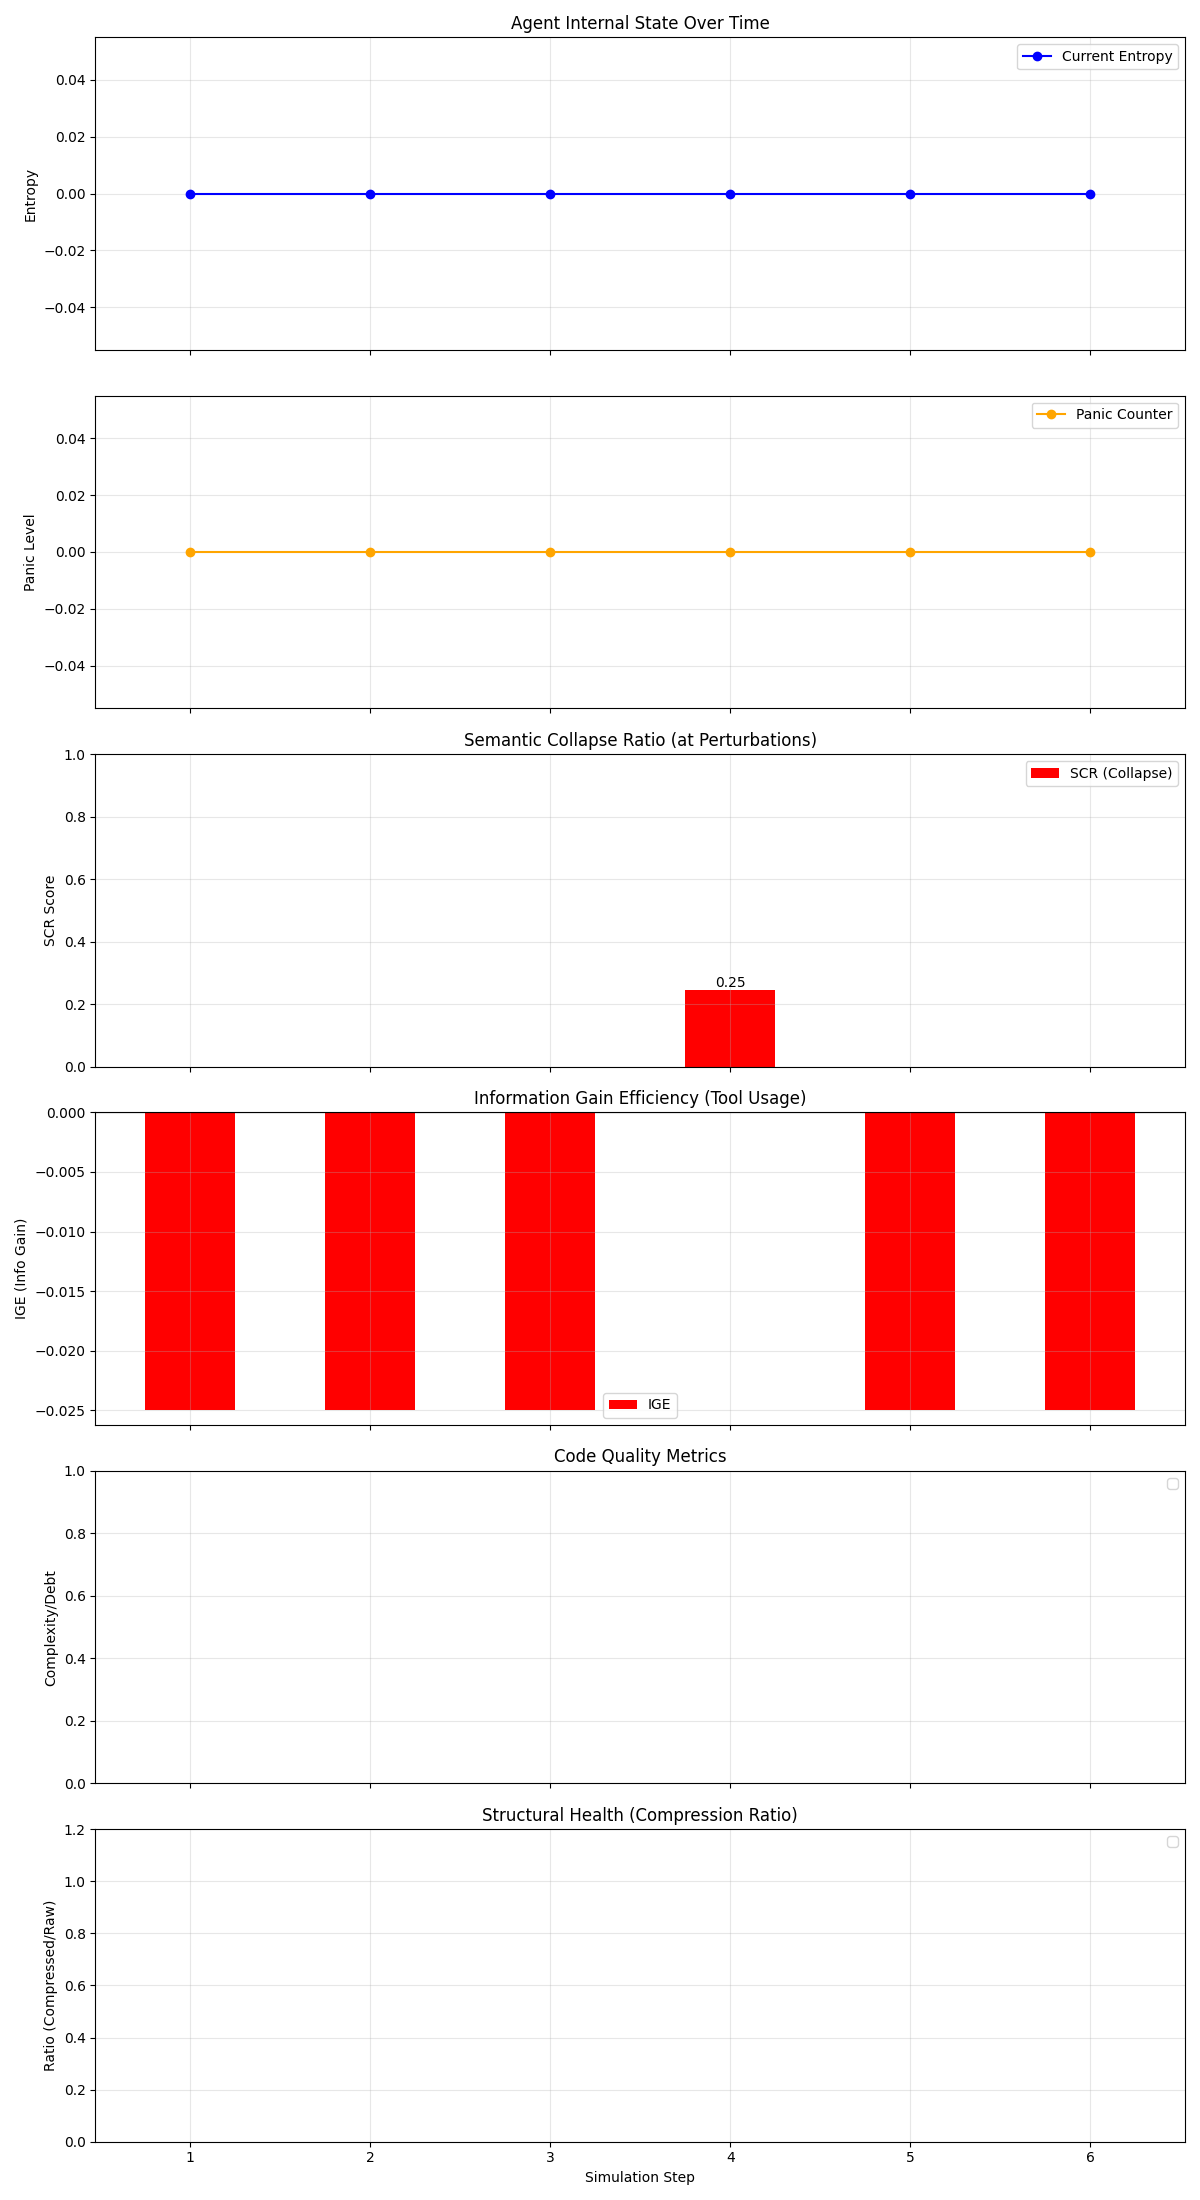
\includegraphics[width=\linewidth]{experiment_summary.png}
  \caption{Experiment Summary. Top to Bottom: (1) Entropy (flatline), (2) Panic Counter, (3) SCR (spikes at shock), (4) IGE, (5) Code Complexity, (6) Compression Ratio.}
\end{figure}

\subsection{Current Evidence (Existing Logs, No New Runs)}
Because new experiments are currently blocked, we summarize \textbf{existing logs} only. We scanned all available JSONL logs and aggregated metadata into \texttt{data/results/existing\_runs\_summary.csv} ($N=71$ runs). Of these, \textbf{21 runs include SCR probes} and \textbf{50 runs are no-probe} (SCR unavailable).

\textbf{Probed runs (SCR available):}
\begin{table}[ht]
  \centering
  \small
  \begin{tabular}{lrrrl}
    \toprule
    Scenario & Steps & Peak SCR & Entropy Cov. & Log \\
    \midrule
    data\_pipeline\_shock & 60 & 0.124 & 0.54 & \texttt{tb\_monitor\_20260105\_231033\_997120.jsonl} \\
    drug\_filter\_shock & 60 & 0.116 & 0.57 & \texttt{tb\_monitor\_20260105\_223229\_992630.jsonl} \\
    hard\_socket\_challenge & 50 & 0.790 & 1.00 & \texttt{tb\_monitor\_20251220\_155717.jsonl} \\
    dirty\_data\_challenge & 43 & 0.789 & 1.00 & \texttt{tb\_monitor\_20251221\_113918.jsonl} \\
    startup\_acquisition\_challenge & 41 & 0.714 & 1.00 & \texttt{tb\_monitor\_20251221\_170148.jsonl} \\
    legacy\_refactor\_challenge & 25 & 0.721 & 1.00 & \texttt{tb\_monitor\_20251218\_230512.jsonl} \\
    hard\_coding\_challenge & 24 & 0.636 & 0.00 & \texttt{tb\_monitor\_20260106\_092340\_209163.jsonl} \\
    \bottomrule
  \end{tabular}
  \caption{Probed runs with SCR available (selected).}
\end{table}

\textbf{Long no-probe runs (SCR unavailable, loop signals visible):}
\begin{table}[ht]
  \centering
  \small
  \begin{tabular}{lrrrl}
    \toprule
    Scenario & Steps & Min Compression & Entropy Cov. & Log \\
    \midrule
    full\_stack\_challenge & 200 & 0.026 & 0.00 & \texttt{tb\_monitor\_20260106\_050534\_094984.jsonl} \\
    dirty\_data\_challenge & 200 & 0.013 & 0.00 & \texttt{tb\_monitor\_20260106\_032337\_528833.jsonl} \\
    hard\_socket\_challenge & 200 & 0.090 & 0.00 & \texttt{tb\_monitor\_20260106\_022602\_395608.jsonl} \\
    hard\_analysis\_challenge & 200 & 0.044 & 0.00 & \texttt{tb\_monitor\_20260106\_013357\_268573.jsonl} \\
    hard\_coding\_challenge & 200 & 0.018 & 0.00 & \texttt{tb\_monitor\_20260105\_234746\_694796.jsonl} \\
    data\_pipeline\_shock & 60 & 0.369 & 0.00 & \texttt{tb\_monitor\_20251231\_135534\_396962.jsonl} \\
    drug\_filter\_shock & 60 & 0.357 & 0.00 & \texttt{tb\_monitor\_20251231\_130200\_286313.jsonl} \\
    \bottomrule
  \end{tabular}
  \caption{Long no-probe runs showing compression ratio collapse (selected).}
\end{table}

\textbf{Interpretation (preliminary):}
\begin{itemize}
  \item SCR spikes appear in probed runs around perturbations, while entropy coverage varies widely (0.00 to 1.00).
  \item In long no-probe runs, compression ratio collapses ($<0.2$) and stays low, indicating severe looping even when entropy is unavailable.
  \item This supports the claim that stability diagnostics must remain informative without logprobs, and that SCR (when available) complements loop-based signals.
\end{itemize}

\section{Related Work}
We position this work relative to: (1) tool-using agent benchmarks, (2) long-horizon context management, and (3) agent failure taxonomies. Our focus is not a new agent policy, but a reproducible \textit{stress-test} harness for non-stationary objectives plus robust observability metrics when common confidence signals are missing.

\textbf{TODO:} finalize citations from \texttt{docs/references.bib} and add canonical references for CoT/ReAct/agent benchmarks used in the experimental design.

\section{Discussion \& Future Work}
Active probing introduces costs and rate-limit pressure; our implementation supports configurable probe modes (off / shock-only / periodic) to study this trade-off. A practical limitation is that branching probes can stress free-tier API limits and require careful throughput planning.

\textbf{Future Work includes:}
\begin{enumerate}
  \item \textbf{Repo repair scenarios:} extend deterministic validators to multi-file codebases with unit tests.
  \item \textbf{Context interventions:} compare model handoff vs context pruning/summarization policies under the same perturbation schedule.
  \item \textbf{Ablations:} probe branch count, embedding model choice for SCR, and budget/cost trade-offs.
\end{enumerate}

\section{Conclusion}
We propose a reproducible framework for evaluating tool-using LLM agents under non-stationary constraints. The key practical contribution is robust observability when token-level confidence is unavailable: SCR probes and outcome-based validators remain informative across heterogeneous providers. This enables paper-ready benchmark tables that measure both \textit{success} and \textit{stability under shocks}.

\section*{References}
References will be finalized from \texttt{docs/references.bib} in the camera-ready version.

\end{document}
